\section{Architecture matérielles des GPUs}
%1
\begin{frame}
    \frametitle{Architecture matérielle}
\begin{block}{Les multiprocesseurs de flux (SM)}
   \begin{itemize}
    \item<+-> Héritier du pipeline graphique, le \textbf{multiprocesseur de flux} ("Streaming multiprocessor", SM) 
    est une entité de traitement comportant des \textbf{séquenceurs}, plusieurs \textbf{unités de traitement numérique}, et une \textbf{mémoire locale}.
    \item<+-> Un processeur graphique (GPU) regroupe plusieurs multiprocesseurs. 
    \item<+-> Les multiprocesseurs exécutent du code de façon \textbf{indépendante} et peuvent accéder à
    une mémoire globale.
    \item<+-> Pour un développeur sur une architecture conventionnelle, un multiprocesseur s'apparente à un c{\oe}ur de calcul
    vectoriel.
   \end{itemize}
\end{block}
    

\end{frame}
%2
\begin{frame}
    \frametitle{Architecture matérielle}
\begin{block}{Les multiprocesseurs de flux (SM)}
   \begin{itemize}
    \item<+->À l'intérieur d'un multiprocesseur, les processus s'exécutent de façon concurrente, mais peuvent communiquer
    via la mémoire locale ou être synchronisés.
    \item<+->Les processus sont répartis en groupes, appelés "warps" (chaînes), qui se voient affecter le même séquenceur 
    d'instructions.
    \item<+->Le modèle associé est dit "SIMT" pour "Single Instruction Multiple Thread".
   \end{itemize} 
\end{block}
\end{frame}
%3
\begin{frame}
    \frametitle{Architecture matérielle}
\begin{block}{Les unités de calcul}
   \begin{itemize}
    \item<+-> Le nombre d'unités de calcul par multiprocesseur dépend des générations de cartes. Pour l'architecture 
    Ampère, on trouve 64 ou 128 unités flottantes 32bits, 32 ou 64 unités flottantes 64bits, 64 unités de calcul entier
    sur 32 bits, 16 unités spéciales (fonctions transcendantes), 4 cœurs de calcul tensoriel et 4 ordonnanceurs.
    \item<+-> Un ordonnanceur est affecté à une chaîne. Tous les processus de la chaîne exécutent la même instruction
    au même moment.
    \item<+-> En cas de branchement, il peut y avoir divergence de code à l'intérieur d'une chaîne, ce qui se traduit par la 
    mise en attente d'un ou plusieurs processus dont l'exécution se poursuivra après celle de la branche principale. 
   \end{itemize} 
\end{block}
\end{frame}

\begin{frame}
    \frametitle{Architecture matérielle}
\begin{block}{L'ordonnancement des processus}
   \begin{itemize}
    \item<+-> Le code à exécuter sur le GPU est appelé noyau ("kernel".)
    \item<+-> Le programmeur décide du nombre de processus affectés à un même noyau et les répartit en blocs.
    \item<+-> Un bloc sera pris en charge par un multiprocesseur libre.
    \item<+-> Dans un bloc, des chaînes de 32 processus identifiés par des entiers consécutifs sont constituées. 
    \item<+-> Depuis l'architecture Volta, chaque processus possède ses propres compteur de programme et pile d'appel,
    ce qui permet un contrôle plus fin, en particulier en cas de divergence.
   \end{itemize} 
\end{block}
\end{frame}
%4

\begin{frame}
    \frametitle{Architecture matérielle}
\begin{block}{L'ordonnancement des processus}
    \begin{figure}[htbp]
        \centering
         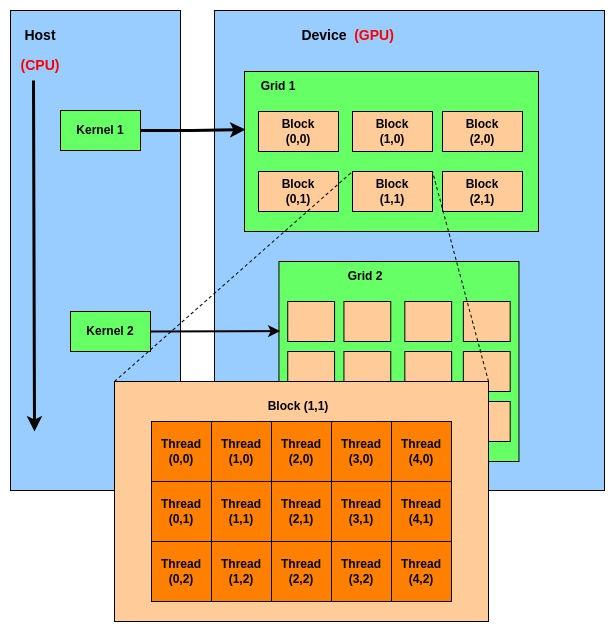
\includegraphics[scale=0.3]{images/ProgrammingModel.jpg} 
        \caption{Modèle de programmation.}
        \label{fig:gforce8}
    \end{figure}
\end{block}
\end{frame}

\begin{frame}
    \frametitle{Architecture matérielle}
\begin{block}{La mémoire}
   \begin{itemize}
    \item<+-> Chaque multiprocesseur possède une mémoire locale très rapide, pouvant être partagée entre les processus
    d'un même bloc. Elle est organisée en 32 banques pouvant être utilisées simultanément. Idéalement, 
    chaque processus d'une chaîne accède à sa propre banque. La capacité de cette mémoire varie entre 64kB et 228kB 
    selon les générations.
    \item<+-> Les multiprocesseurs partagent une mémoire globale, plus lente, mais en mesure de stocker beaucoup plus 
    de données. Les cartes de dernière génération, comme la RTX4090, embarquent 24Gb de RAM.
    \item<+-> L'architecture 9.0 introduit la notion de cluster de blocs et de mémoire partagée distribuée.
   \end{itemize} 
\end{block}
\end{frame}
\begin{frame}{Les mémoires spécialisées}
\begin{block}{La mémoire de textures}
   \begin{itemize}
    \item<+-> Les GPUs étant initialement conçus pour des applications de rendu graphique 3D, certaines mémoires
    dédiées sont présentes. 
    \item<+-> La mémoire de textures est particulièrement intéressante lorsque l'on cherche à stocker des données
    bidimensionnelles que l'on souhaite ensuite interpoler.
    \item<+-> Cette mémoire, chargée par le CPU, ne peut être modifiée par un programme CUDA.
   \end{itemize} 
\end{block}
\end{frame}

\begin{frame}{Les mémoires spécialisées}
\begin{block}{Architecture d'une grille.}
    \begin{figure}[htbp]
        \centering
         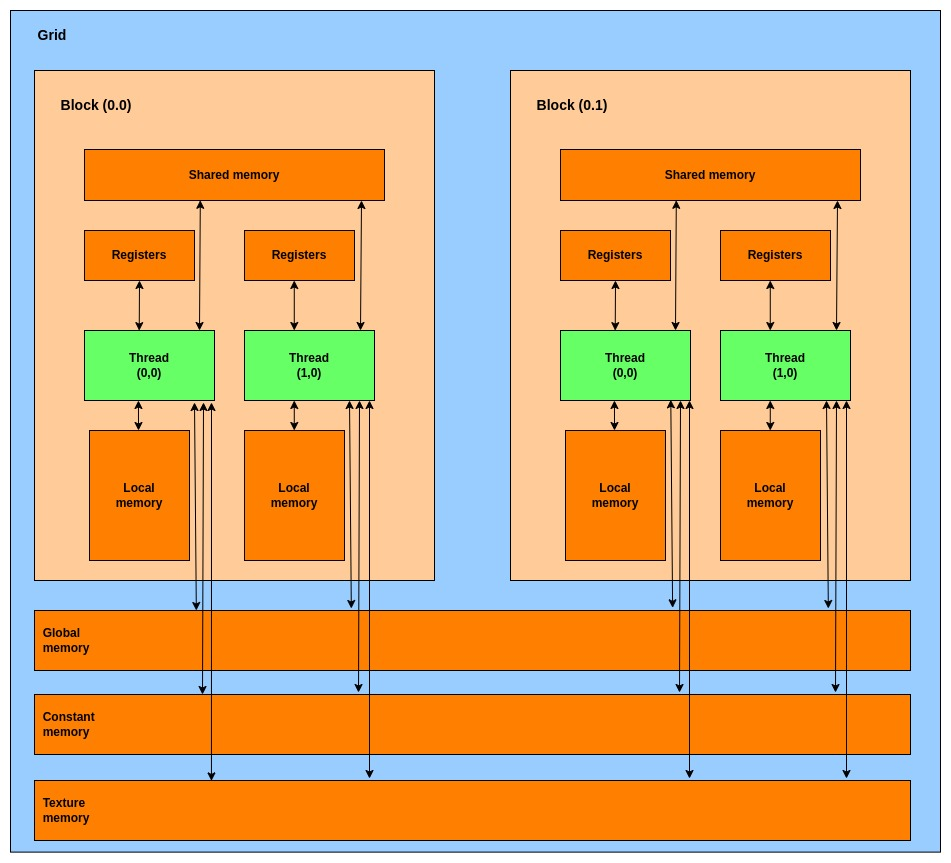
\includegraphics[scale=0.2]{images/ArchitectureGridCUDA.jpg} 
        \caption{Architecture d'une grille.}
        \label{fig:gforce8}
    \end{figure}
\end{block}
\end{frame}

\begin{frame}{\`A retenir}
\begin{block}{Le GPU}
   \begin{itemize}
    \item<+-> Un bloc est affecté à un multiprocesseur, les processus d'une même chaîne exécutent la même instruction
    en parallèle.
    \item<+-> Il faut donc penser avant tout en termes de chaînes (32 processus).
   \end{itemize} 
\end{block}
\begin{block}{La mémoire}
  \begin{itemize}
   \item<+-> Privilégier l'utilisation de la mémoire partagée, bien plus rapide que la mémoire globale.
   \item<+-> S'efforcer d'avoir des accès contigus pour les processus d'une même chaîne.
   \item<+-> Utiliser la mémoire des textures si nécessaire.
  \end{itemize} 
\end{block}
\end{frame}
